\section{Preliminary Results and Findings}
\label{sec:preliminary_results}

This section presents the results obtained from training a subset of the algorithms discussed in section \ref{subsec:algorithm_selection}. The selected algorithms include five DQN-based methods — DQN, Double DQN, Prioritized Experience Replay, Dueling DQN, and C51 — as well as three policy-based methods: REINFORCE, PPO, and SAC. Soft Actor Critic was preferred to DDPG and TD3 because it can simply be seen as a variation that works with a stochastic policy, but is more easily adapted to a discrete action space.

We first describe necessary modifications to the experiment setup, followed by a detailed analysis of each algorithm's performance and emissions. The results are then compared across different algorithm families.

\subsection{Experiment Setup Adjustments}
\label{subsec:exp_setup_adjustments}
During initial training attempts, some adjustments were required to ensure reliable performance and energy tracking. One key reason for this was that employing CodeCarbon as a (next-)real-time emissions tracking tool significantly slowed down training (by a factor of 20 or more). As a result, we opted to record only total emissions at the end of training rather than tracking them continously. This adjustment allowed us to obtain meaningful comparisons without excessively increasing training time.

In addition to this, on Windows, CodeCarbon's CPU energy tracking relies on the Intel Power Gadget, which has been deprecated for several years. Furthermore, it does not support Intel Performance Counter Monitor (Intel PCM), the official successor to the Power Gadget. In such cases, CodeCarbon switches to a fallback mode, directly quoting from their documentation:
\begin{quoting}
	\begin{itemize}
		\item It will first detect which CPU hardware is currently in use, and then map it to a data source listing 2000+ Intel and AMD CPUs and their corresponding thermal design powers (TDPs).
		
		\item If the CPU is not found in the data source, a global constant will be applied. CodeCarbon assumes that 50\% of the TDP will be the average power consumption to make this approximation.
		
		\item We could not find any good resource showing statistical relationships between TDP and average power, so we empirically tested that 50\% is a decent approximation.
	\end{itemize}
\end{quoting}

This approach should provide reasonable estimates for our project, since most of the workload is on the GPU, while the rest is mostly constant across the algorithms (like the environment simulations). This being said, one instance where this limitation may have had an impact is in tracking the Proximal Policy Optimization (PPO) algorithm, that employs a relatively small neural network but requires more CPU and RAM processing, the latter also explicitly stated to not be tracked satisfactorily.

Moreover, wandb collect systems data, but it also, while collecting kwh for the gpu, does not for cpu and ram, so we have to make do with what we have

Additionally, Weights \& Biases collects system data during training, and while it tracks GPU energy consumption in kWh, it also does not do the same for CPU and RAM. As a result, while we can obtain excellent emissions estimates for the GPU, CPU and RAM energy tracking remains imprecise due to the aforementioned limitations. Consequently, energy consumption analyses must be interpreted with an understanding of these constraints.

\subsection{DQN-Based Algorithms}
We present the results for the five different DQN-based algorithms. Each algorithm is analyzed individually before an overall comparison.

\subsubsection{Deep Q-Network (DQN Baseline)}
\label{subsubsec:dqn_baseline}

\paragraph{(Hyper)Parameters.}
Table~\ref{tab:dqn_hyperparams} summarizes the main hyperparameters used for our DQN baseline.  
\texttt{env\_id} and \texttt{seed} varied across runs (eight Atari games $\times$ four seeds), 
while the rest remained unchanged. Note in particular that \texttt{buffer\_size} and 
\texttt{learning\_starts} have been reduced relative to their usual millions-step values to 
accommodate the shorter 100k-step regime.

\begin{table}%[htbp]
	\caption{Key hyperparameters for the DQN baseline. Only \texttt{env\_id} and \texttt{seed} change across runs.}
	\label{tab:dqn_hyperparams}
	\centering
	\begin{tabular}{ll}
		\toprule
		\textbf{Parameter} & \textbf{Value} \\
		\midrule
		\texttt{exp\_name}                & dqn\_atari \\
		\texttt{seed}                     & 1..4 \\
		\texttt{torch\_deterministic}     & True \\
		\texttt{cuda}                     & True \\
		\texttt{track}                    & True \\
		\texttt{wandb\_project\_name}     & rlsb \\
		\texttt{capture\_video}           & False \\
		\texttt{save\_model}              & True \\
		\texttt{upload\_model}            & False \\
		\texttt{env\_id}                  & e.g.\ AlienNoFrameskip-v4 \\
		\texttt{total\_timesteps}         & 100000 \\
		\texttt{learning\_rate}           & 0.0001 \\
		\texttt{num\_envs}                & 1 \\
		\texttt{buffer\_size}             & 10000 \\
		\texttt{gamma}                    & 0.99 \\
		\texttt{tau}                      & 1.0 \\
		\texttt{target\_network\_frequency} & 1000 \\
		\texttt{batch\_size}             & 32 \\
		\texttt{start\_e}, \texttt{end\_e} & 1.0 $\to$ 0.01 \\
		\texttt{exploration\_fraction}    & 0.1 \\
		\texttt{learning\_starts}         & 1000 \\
		\texttt{train\_frequency}         & 4 \\
		\bottomrule
	\end{tabular}
\end{table}

\paragraph{Hyperparameter Tuning}
We began with the \emph{CleanRL} defaults (similar to Mnih~et~al.'s original DQN~\cite{mnih:atari}) and
scaled down parameters tied to a large number of environment interactions. For instance,
\texttt{buffer\_size} was tested at \{10k, 20k\}, and \texttt{learning\_starts} 
at \{800, 1000, 2000, 5000\}. Empirically, a buffer of 10k 
and \texttt{learning\_starts} of 1000 provided the best trade-off between stability 
and performance in the 100k-step setting. We kep $\tau$ equal to \num{1} for consistency with the original work.
This parameter regulates the update of the target network weights by controlling the interpolation between those of the 
current Q-network and target network, following the update rule:
$$
\theta_{\text{target}} = \tau \theta + (1 - \tau) \theta_{\text{target}}
$$
where $\theta_{\text{target}}$ are the weights of the target network and $\theta$ are the ones of the q-network.
For \(\tau = 1\), the target network is completely overwritten by the Q-network 
every time it's updated, as done in the original DQN.

\paragraph{Training Dynamics (Aggregated Over 32 Runs)}
Figure~\ref{fig:dqn_episodic_length} shows that episodes usually last in the 3000--4000 step range, 
but certain runs or environments have early terminations (very short episodes) or extremely long ones (around 8000 steps).  
Figure~\ref{fig:dqn_sps} indicates that, computationally, training stabilizes at a solid 
\(\sim\)170 steps per second on average, though hardware and environment differences 
introduce notable variance.

\begin{figure}
	\centering
	\subfloat[][\emph{Aggregated episodic length for DQN over 100k steps (interpolation across 32 runs). 
		The mean hovers around 3500--4000 steps, 
		while the min--max envelope extends from near 0 to over 8000.}]
	{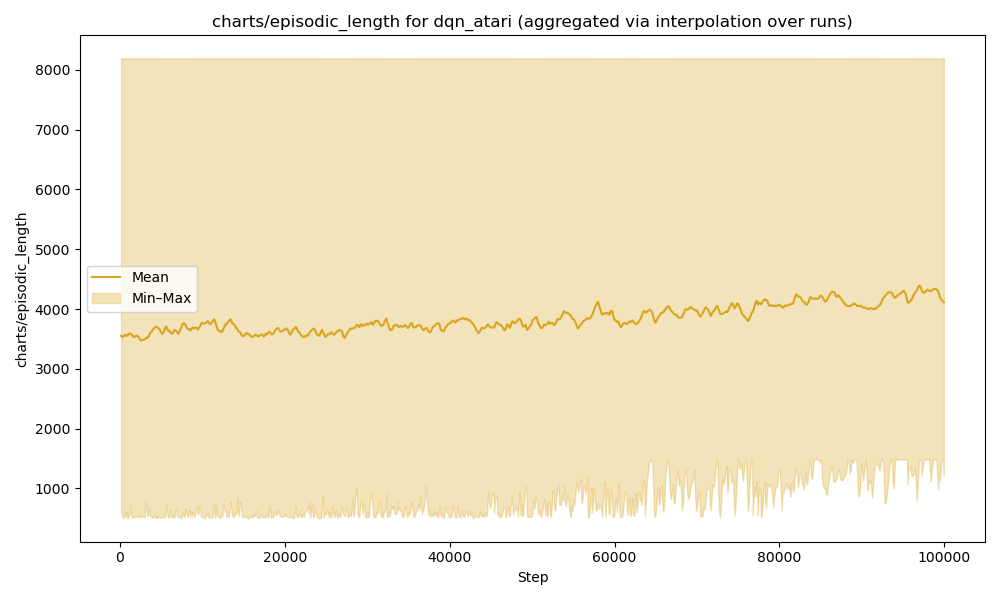
\includegraphics[width=.45\textwidth]{figures/dqn/charts_episodic_length_dqn_atari.png} \label{fig:dqn_episodic_length}} \quad
	\subfloat[][\emph{Steps per second (SPS) for DQN. After an initial ramp-up, 
		the mean SPS stabilizes around 170--180, 
		with some runs dipping as low as 20 or spiking above 200.}]
	{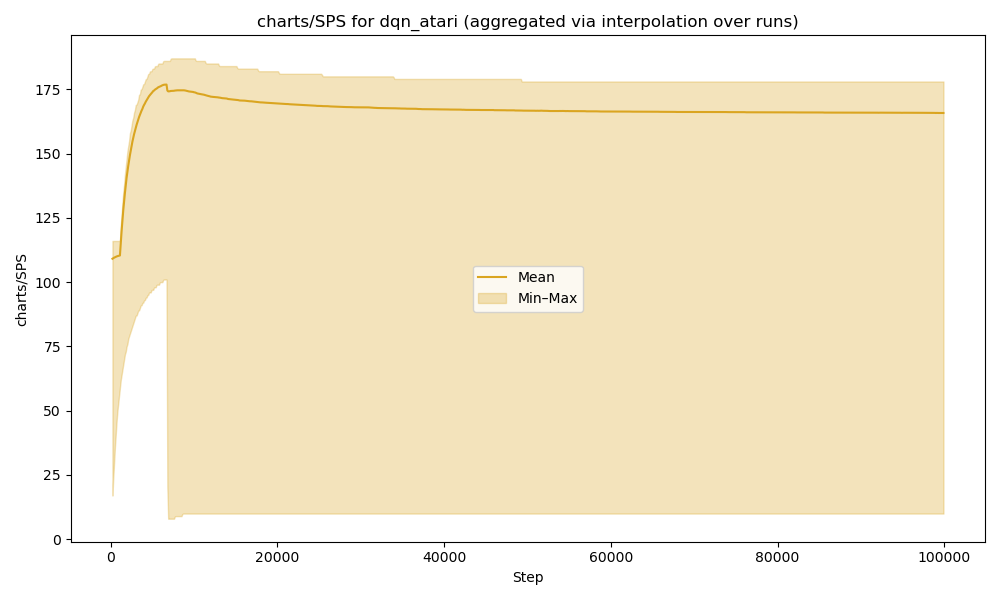
\includegraphics[width=.45\textwidth]{figures/dqn/charts_SPS_dqn_atari.png} \label{fig:dqn_sps}} \\ 
	\subfloat[][\emph{Estimated Q-values (\texttt{losses/q\_values}) for DQN 
		(aggregated over 32 runs). 
		The mean Q-value climbs from near 0 up to \(\sim\)4--5, 
		while some runs exceed 10.}]
	{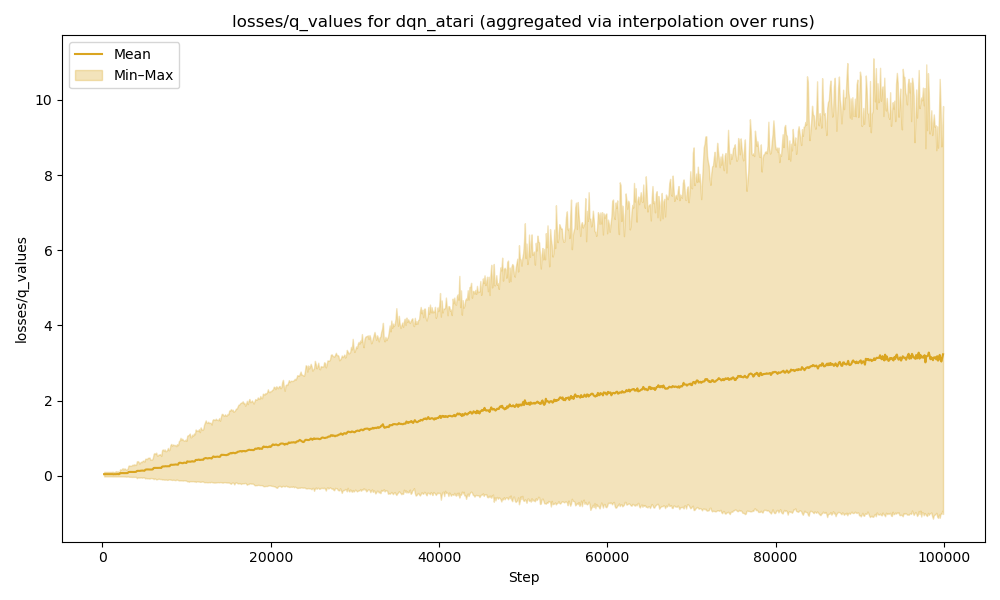
\includegraphics[width=.45\textwidth]{figures/dqn/losses_q_values_dqn_atari.png} \label{fig:dqn_q_values}} \quad
	\subfloat[][\emph{TD loss (\texttt{losses/td\_loss}) for DQN. 
		Losses grow with training, reaching above 3.0 in some runs, 
		reflecting substantial variance near the final stages.}]
	{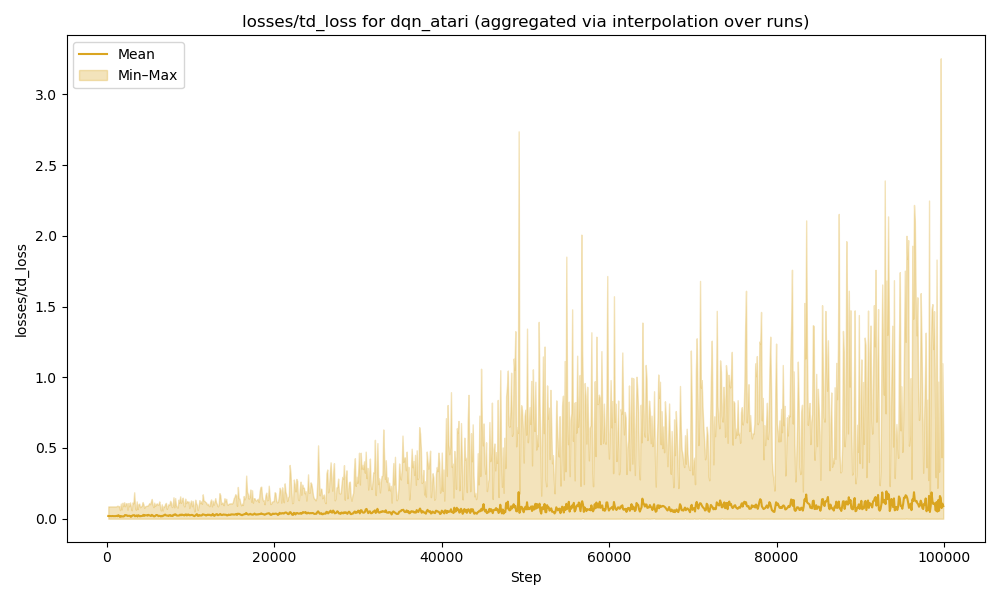
\includegraphics[width=.45\textwidth]{figures/dqn/losses_td_loss_dqn_atari.png} \label{fig:dqn_td_loss}}
	\caption{Performance metrics for DQN over 100k steps, aggregated across 32 runs.}
	\label{fig:dqn_subfigures}
\end{figure}

%
%\begin{figure}
%	\centering
%	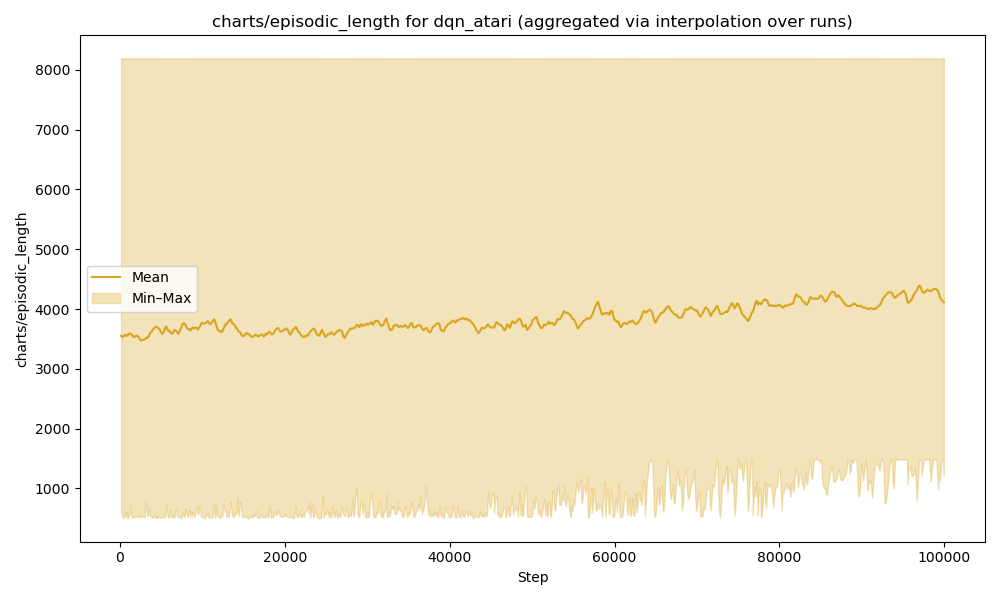
\includegraphics[width=0.6\textwidth]{figures/dqn/charts_episodic_length_dqn_atari.png}
%	\caption{Aggregated episodic length for DQN over 100k steps 
%		(interpolation across 32 runs). 
%		The mean hovers around 3500--4000 steps, 
%		while the min--max envelope extends from near 0 to over 8000.}
%	\label{fig:dqn_episodic_length}
%\end{figure}
%\begin{figure}
%	\centering
%	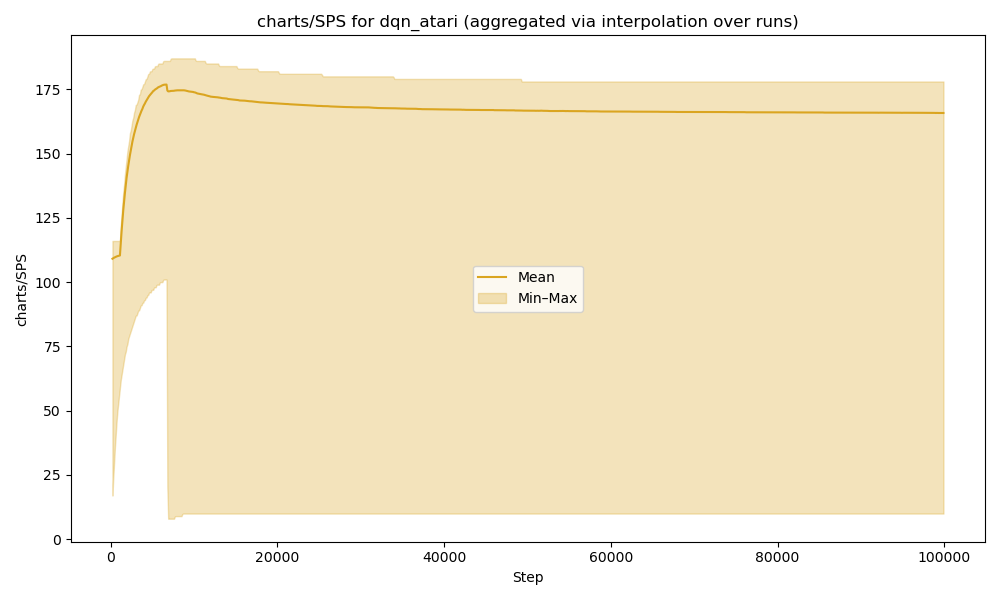
\includegraphics[width=0.6\textwidth]{figures/dqn/charts_SPS_dqn_atari.png}
%	\caption{Steps per second (SPS) for DQN. After an initial ramp-up, 
%		the mean SPS stabilizes around 170--180, 
%		with some runs dipping as low as 20 or spiking above 200.}
%	\label{fig:dqn_sps}
%\end{figure}
%\begin{figure}
%	\centering
%	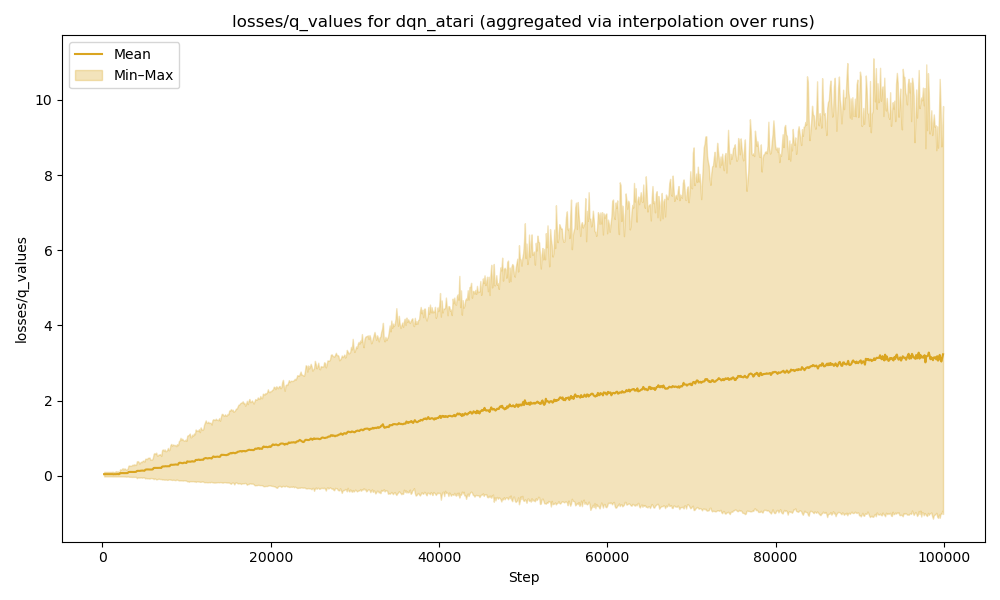
\includegraphics[width=0.6\textwidth]{figures/dqn/losses_q_values_dqn_atari.png}
%	\caption{Estimated Q-values (\texttt{losses/q\_values}) for DQN 
%		(aggregated over 32 runs). 
%		The mean Q-value climbs from near 0 up to \(\sim\)4--5, 
%		while some runs exceed 10.}
%	\label{fig:dqn_q_values}
%\end{figure}
%\begin{figure}
%	\centering
%	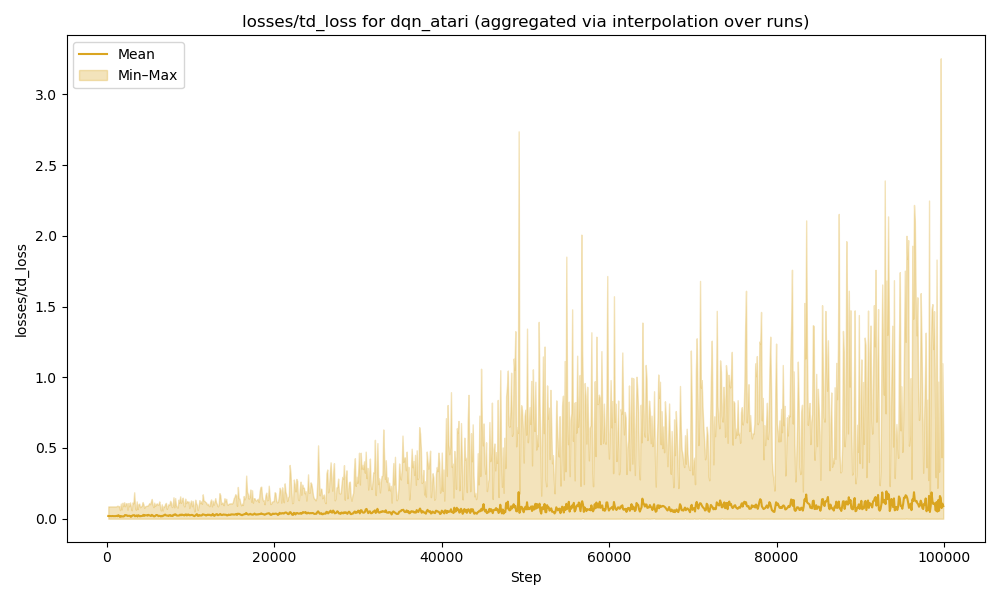
\includegraphics[width=0.6\textwidth]{figures/dqn/losses_td_loss_dqn_atari.png}
%	\caption{TD loss (\texttt{losses/td\_loss}) for DQN. 
%		Losses grow with training, reaching above 3.0 in some runs, 
%		reflecting substantial variance near the final stages.}
%	\label{fig:dqn_td_loss}
%\end{figure}

\paragraph{Q-Values and TD Loss.}
Figures~\ref{fig:dqn_q_values} and \ref{fig:dqn_td_loss} show \texttt{losses/q\_values} and 
\texttt{losses/td\_loss}, respectively, across all runs.
On average, Q-values increase steadily, suggesting the network’s estimates 
of future returns keep growing with experience. However, 
the broad min--max band indicates some seeds or games diverge or plateau differently. 
The TD loss remains small in early training but spikes in certain runs, 
possibly due to volatile updates from the replay buffer once it’s partially filled.

\paragraph{Episodic Return (Human vs.\ Min--Max Normalized).}
We analyzed the collected episodic returns applying both the human normalization and min--max normalization schemes, as explained in section~\vref{subsubsec:normalization}.
Figures~\ref{fig:dqn_return_human} and \ref{fig:dqn_return_minmax} aggregate 
these returns across all 32 runs, while 
Figures~\ref{fig:dqn_return_pergame_human} and \ref{fig:dqn_return_pergame_minmax} 
show per-game curves.

\begin{figure}
	\centering
	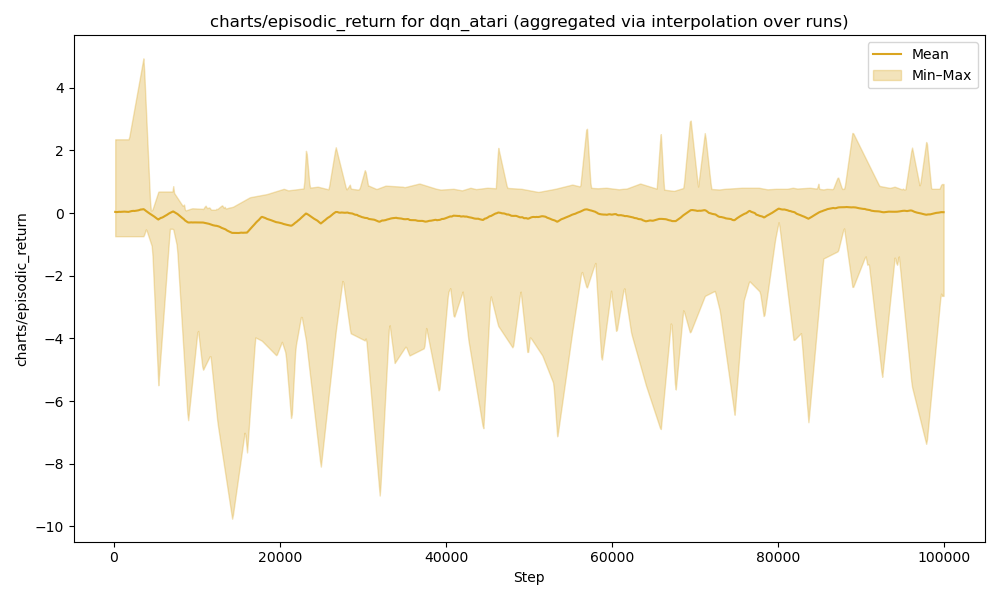
\includegraphics[width=0.6\textwidth]{figures/dqn/charts_episodic_return_human_dqn_atari.png}
	\caption{Aggregated DQN episodic return (human-normalized) 
		over 100k steps. The shaded region represents min--max variation.}
	\label{fig:dqn_return_human}
\end{figure}

\begin{figure}
	\centering
	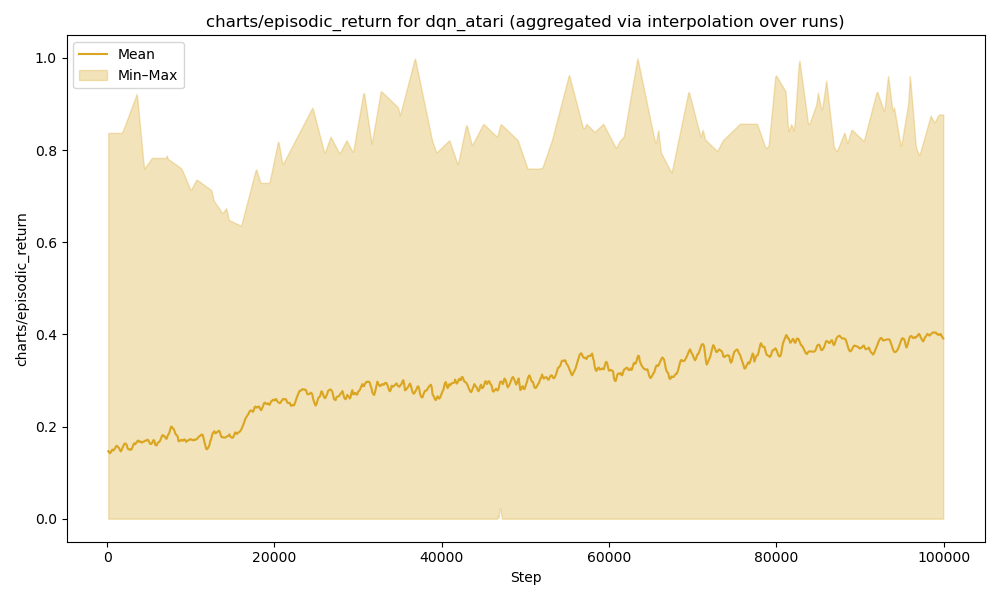
\includegraphics[width=0.6\textwidth]{figures/dqn/charts_episodic_return_minmax_dqn_atari.png}
	\caption{Aggregated DQN episodic return (min--max normalized).}
	\label{fig:dqn_return_minmax}
\end{figure}

In the human-normalized plot, the mean hovers near zero, 
occasionally dipping negative due to poor performance on certain games. 
In the min--max plot, the average climbs from near 0.2 to around 0.4--0.5 by the end, 
indicating moderate relative progress.

\begin{figure}
	\centering
	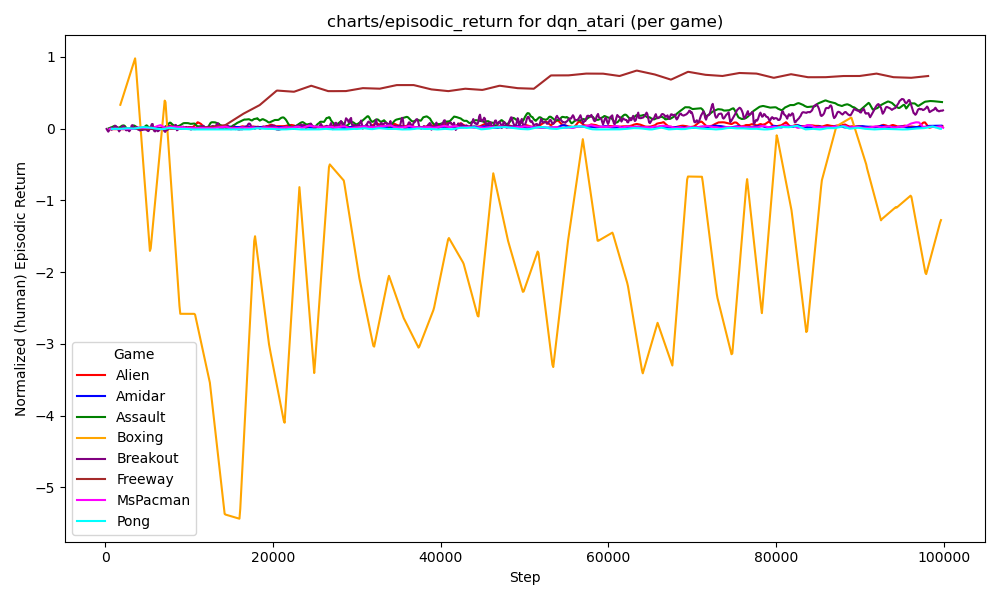
\includegraphics[width=0.6\textwidth]{figures/dqn/charts_episodic_return_per_game_human_dqn_atari.png}
	\caption{DQN returns (human-normalized) by game. Each line aggregates 
		four seeds for that specific environment.}
	\label{fig:dqn_return_pergame_human}
\end{figure}

\begin{figure}
	\centering
	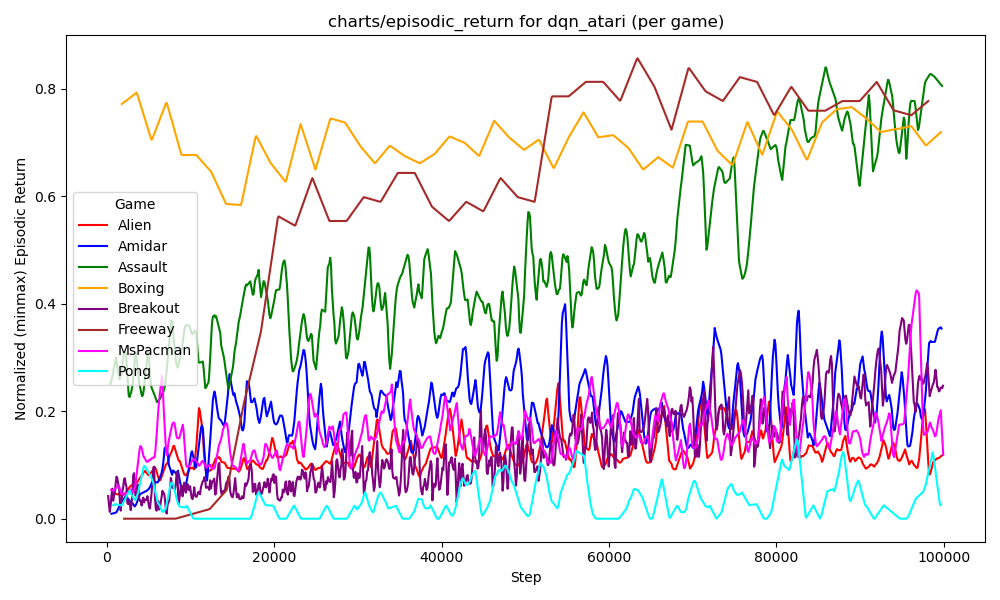
\includegraphics[width=0.6\textwidth]{figures/dqn/charts_episodic_return_per_game_minmax_dqn_atari.png}
	\caption{DQN returns (min--max normalized) by game.}
	\label{fig:dqn_return_pergame_minmax}
\end{figure}

Different environments see dramatically different results: 
\emph{Freeway} often approaches high normalized scores, while 
\emph{Pong} and \emph{MsPacman} remain relatively low 
(especially in the human-normalized scale).

\paragraph{Emissions}
Table~\ref{tab:dqn_emissions} presents the aggregated CO\textsubscript{2}-eq for DQN 
(over all 32 runs). The mean is about \(\textbf{0.00647 kg}\), 
with a minimum of 0.00616 and a maximum near 0.0070.

\begin{table}
	\caption{Carbon emissions (kg\,CO\textsubscript{2}eq) for DQN across 32 runs.}
	\label{tab:dqn_emissions}
	\centering
	\makebox[\textwidth]{%
	\begin{tabularx}{1.1\textwidth}{lXXXXXXXX}
		\toprule
		\textbf{Algorithm} & \textbf{mean} & \textbf{std} & \textbf{median} & 
		\textbf{q25} & \textbf{q75} & \textbf{min} & \textbf{max} & \textbf{iqmean} \\
		\midrule
		DQN & 0.006469 & 0.0002609 & 0.006342 & 0.006296 & 0.006578 & 0.006162 & 0.006997 & 0.006369 \\
		\bottomrule
	\end{tabularx}
	}
\end{table}

\paragraph{Evaluation Results}
Table~\ref{tab:dqn_eval_overall} aggregates final human-/min--max-normalized 
returns \emph{over all 32 runs}. A game-by-game breakdown 
(Table~\ref{tab:dqn_eval_gamewise}) highlights large variability: 
\emph{Freeway} can exceed 0.7 (human norm) or 0.75 (min--max), 
while \emph{Boxing} sees a wide range from $-5$ to nearly $+5$ in human norm.

\begin{table}
	\caption{Overall final evaluation (10 episodes each) for DQN across all runs.}
	\label{tab:dqn_eval_overall}
	\centering
	\begin{tabular}{lcccccccc}
		\toprule
		\textbf{Normalization} & \textbf{mean} & \textbf{std} & \textbf{median} & 
		\textbf{q25} & \textbf{q75} & \textbf{min} & \textbf{max} & \textbf{iqmean} \\
		\midrule
		\textbf{Human} & 0.1353 & 0.7541 & 0.0338 & 0.00072 & 0.398 & -5.024 & 4.738 & 0.1137 \\
		\textbf{Min--Max} & 0.3802 & 0.3099 & 0.2899 & 0.0969 & 0.7143 & 0.0 & 0.9881 & 0.3426 \\
		\bottomrule
	\end{tabular}
\end{table}

\begin{table}
	\caption{Per-game final evaluation for DQN (human- vs.\ min--max normalized). 
		Each cell aggregates 10 episodes $\times$ 4 seeds = 40 total episodes in that game.}
	\label{tab:dqn_eval_gamewise}
	\centering
	\begin{tabular}{llcccc}
		\toprule
		\textbf{Game} & \textbf{Norm} & \textbf{mean} & \textbf{std} & \textbf{min} & \textbf{max}\\
		\midrule
		Alien    & Human   & 0.0624 & 0.0752 & 0.0048 & 0.2636 \\
		    & Min--Max & 0.1607 & 0.1250 & 0.0650 & 0.4950 \\
		\cmidrule{1-6}
		Amidar   & Human   & 0.0226 & 0.0138 & 0.00072 & 0.0450 \\
		   & Min--Max & 0.2005 & 0.1065 & 0.0323 & 0.3733 \\
		\cmidrule{1-6}
		Assault  & Human   & 0.3167 & 0.1120 & -0.0262 & 0.4920 \\
		  & Min--Max & 0.7216 & 0.1703 & 0.2005 & 0.9881 \\
		\cmidrule{1-6}
		Boxing   & Human   & -0.4167 & 1.9504 & -5.0238 & 4.7381 \\
		   & Min--Max & 0.7469 & 0.0635 & 0.5969 & 0.9147 \\
		\cmidrule{1-6}
		Breakout & Human   & 0.3796 & 0.1246 & 0.1096 & 0.6080 \\
		 & Min--Max & 0.3454 & 0.0987 & 0.1316 & 0.5263 \\
		\cmidrule{1-6}
		Freeway  & Human   & 0.7162 & 0.0589 & 0.6419 & 0.8784 \\
		  & Min--Max & 0.7571 & 0.0622 & 0.6786 & 0.9286 \\
		\cmidrule{1-6}
		MsPacman & Human   & 0.0099 & 0.0120 & -0.0076 & 0.0262 \\
		 & Min--Max & 0.1047 & 0.0484 & 0.0340 & 0.1702 \\
		\cmidrule{1-6}
		Pong     & Human   & -0.0083 & 0.0074 & -0.01 & 0.0233 \\
		     & Min--Max & 0.0050 & 0.0221 & 0.0 & 0.1 \\
		\bottomrule
	\end{tabular}
\end{table}

\paragraph{Observations.}
In summary:
\begin{itemize}
	\item \textbf{Episodic length} stabilizes around 3500--4000 steps on average, 
	with some extreme runs either terminating quickly or persisting up to 8000 steps.
	\item \textbf{SPS} quickly rises to around 170--180, illustrating the efficiency 
	of the implementation (though some runs are slower).
	\item \textbf{Q-values and TD loss} both exhibit broad variability. On average, 
	Q-values climb steadily to 4--5, but certain runs exceed 10. The TD loss 
	can spike above 3 for some seeds, indicating unstable updates.
	\item \textbf{Returns} show moderate success on easier tasks like \textit{Freeway} 
	and \textit{Boxing}, but remain low in \textit{Pong} or \textit{MsPacman}. Overall, 
	min--max mean is about 0.38, whereas human-normalized is only 0.14 (due in part 
	to highly negative outliers on certain seeds).
	\item \textbf{Emissions} remain modest, at about 0.00647\,kg CO\textsubscript{2}-eq 
	per run. This is unsurprising for a 100k-step budget, but still notable for 
	comparing across algorithms in subsequent sections.
\end{itemize}

DQN thus provides a baseline—relatively simple and lightweight—to which we will 
compare Double DQN, Prioritized Experience Replay, Dueling DQN, and C51 
in the next subsections, evaluating whether each extension justifies 
its additional complexity and energy usage.


\subsubsection{Double DQN}
\label{subsubsec:double_dqn}

\paragraph{(Hyper)Parameters.}
Table~\ref{tab:ddqn_hyperparams} shows the main hyperparameters used in our Double DQN implementation.  
As with the baseline DQN (Section~\ref{subsubsec:dqn_baseline}), \texttt{env\_id} and \texttt{seed} vary across the 32 runs (eight Atari games $\times$ four seeds), while the rest remain unchanged. In particular, we again set \texttt{buffer\_size}=10k and \texttt{learning\_starts}=1000. 
The Double DQN update rule differs from standard DQN by separately selecting the action and evaluating its value, aiming to reduce the maximization bias that arises from using the same values to both choose and evaluate an action.

\begin{table}
	\caption{Key hyperparameters for Double DQN. Only \texttt{env\_id} and \texttt{seed} change across runs.}
	\label{tab:ddqn_hyperparams}
	\centering
	\begin{tabular}{ll}
		\toprule
		\textbf{Parameter} & \textbf{Value} \\
		\midrule
		\texttt{exp\_name}                & ddqn\_atari \\
		\texttt{seed}                     & 1..4 \\
		\texttt{torch\_deterministic}     & True \\
		\texttt{cuda}                     & True \\
		\texttt{track}                    & True \\
		\texttt{wandb\_project\_name}     & rlsb \\
		\texttt{capture\_video}           & False \\
		\texttt{save\_model}              & True \\
		\texttt{upload\_model}            & False \\
		\texttt{env\_id}                  & e.g.\ AlienNoFrameskip-v4 \\
		\texttt{total\_timesteps}         & 100000 \\
		\texttt{learning\_rate}           & 0.0001 \\
		\texttt{num\_envs}                & 1 \\
		\texttt{buffer\_size}             & 10000 \\
		\texttt{gamma}                    & 0.99 \\
		\texttt{tau}                      & 1.0 \\
		\texttt{target\_network\_frequency} & 1000 \\
		\texttt{batch\_size}             & 32 \\
		\texttt{start\_e}, \texttt{end\_e} & 1.0 $\to$ 0.01 \\
		\texttt{exploration\_fraction}    & 0.1 \\
		\texttt{learning\_starts}         & 1000 \\
		\texttt{train\_frequency}         & 4 \\
		\bottomrule
	\end{tabular}
\end{table}

\paragraph{Hyperparameter Tuning.}
To isolate the effect of Double DQN, we kept all settings identical to the baseline DQN, simply enabling the Double DQN update scheme. 
Following \cite{van:double_q}, we tested a higher \texttt{target\_network\_frequency} (e.g.\ 3000, scaled from the 10k--20k range in the original paper), but at 100k steps, performance was comparable or slightly better with 1000, so we retained the lower frequency. 

\paragraph{Training Dynamics (Aggregated Over 32 Runs).}
Figure~\ref{fig:ddqn_subfigs} presents key metrics—episodic length, steps per second (SPS), estimated Q-values, and TD loss—aggregated across 32 runs (eight games, four seeds each). 

\begin{figure}
	\centering
	\subfloat[][Episodic length (\texttt{charts\_episodic\_length}). 
	The mean sits around 3500--4000 steps, 
	min--max ranges from near 0 up to 8000.]{
		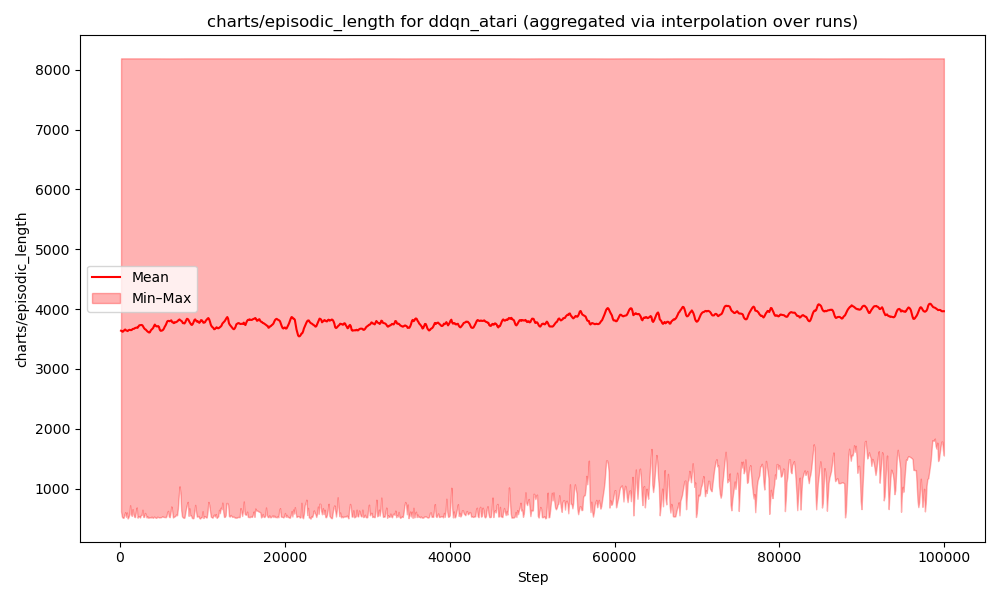
\includegraphics[width=.45\textwidth]{figures/ddqn/charts_episodic_length_ddqn_atari.png}
		\label{fig:ddqn_episodic_length}
	}
	\quad
	\subfloat[][Steps per second (SPS). After an initial climb near 180, 
	the mean gradually settles around 165--170.]{
		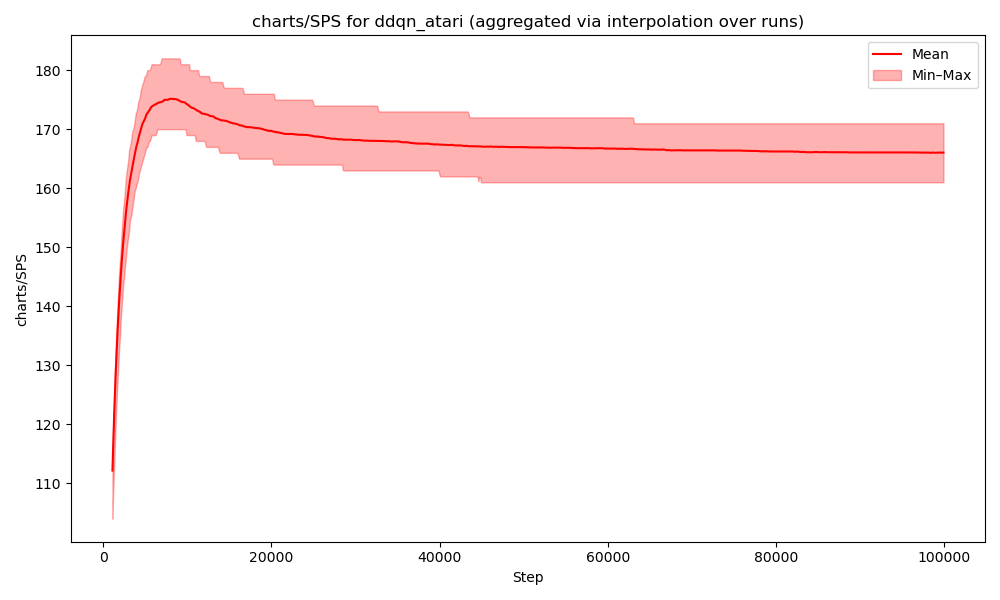
\includegraphics[width=.45\textwidth]{figures/ddqn/charts_SPS_ddqn_atari.png}
		\label{fig:ddqn_sps}
	}
	\\[1em]
	\subfloat[][Estimated Q-values (\texttt{losses/q\_values}). 
	The mean climbs from 0 to about 2--3, 
	with upper outliers above 6.]{
		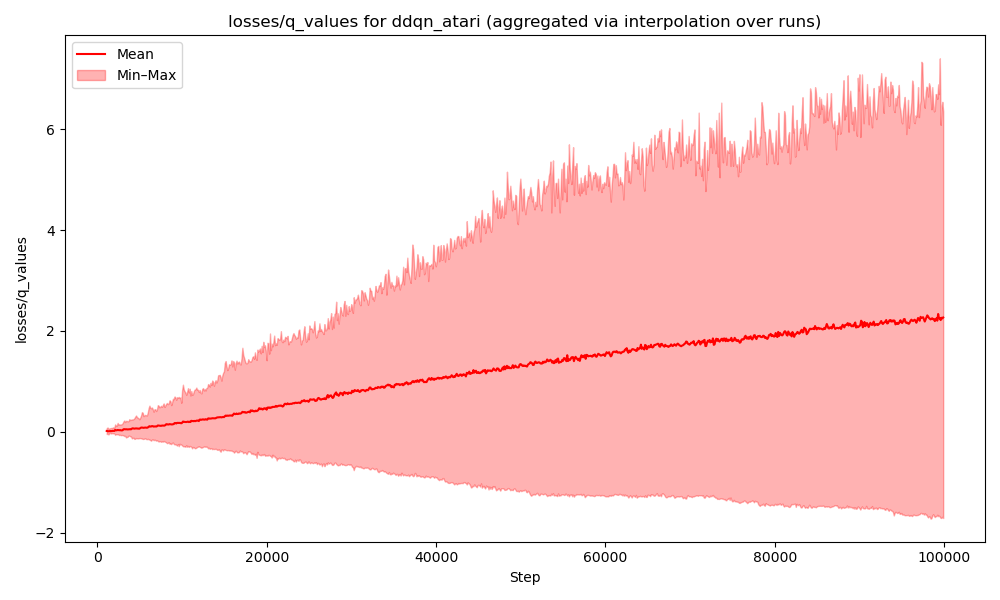
\includegraphics[width=.45\textwidth]{figures/ddqn/losses_q_values_ddqn_atari.png}
		\label{fig:ddqn_q_values}
	}
	\quad
	\subfloat[][TD loss (\texttt{losses/td\_loss}). 
	Occasional spikes above 2.0 reflect instability on certain seeds.]{
		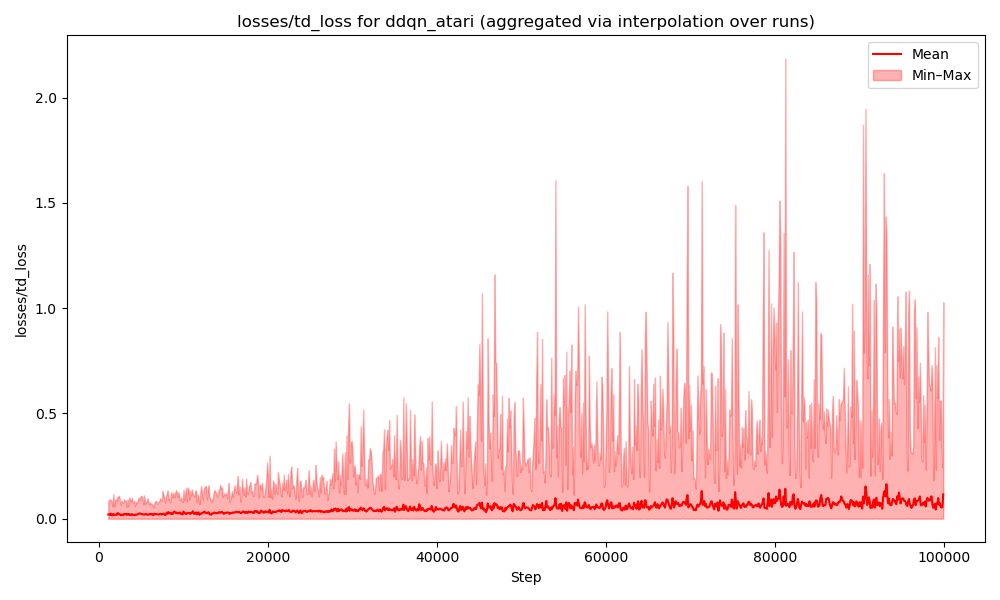
\includegraphics[width=.45\textwidth]{figures/ddqn/losses_td_loss_ddqn_atari.png}
		\label{fig:ddqn_td_loss}
	}
	\caption{Double DQN training metrics over 100k steps, aggregated over 32 runs.}
	\label{fig:ddqn_subfigs}
\end{figure}

Episodic length and SPS curves are very similar to baseline DQN’s (Section~\ref{subsubsec:dqn_baseline}). 
Meanwhile, the mean Q-values grow more modestly than DQN’s (which often exceed 4--5 by the end), suggesting 
Double DQN’s approach does mitigate overestimation somewhat. 
TD loss remains low overall, though some runs spike above 2.0 near late training.

\paragraph{Episodic Return (Human vs.\ Min--Max Normalized).}
Figures~\ref{fig:ddqn_return_human} and \ref{fig:ddqn_return_minmax} show Double DQN’s aggregated episodic returns (human- and min--max-normalized, respectively). 
Figures~\ref{fig:ddqn_return_pergame_human} and \ref{fig:ddqn_return_pergame_minmax} break these results down by game.

\begin{figure}
	\centering
	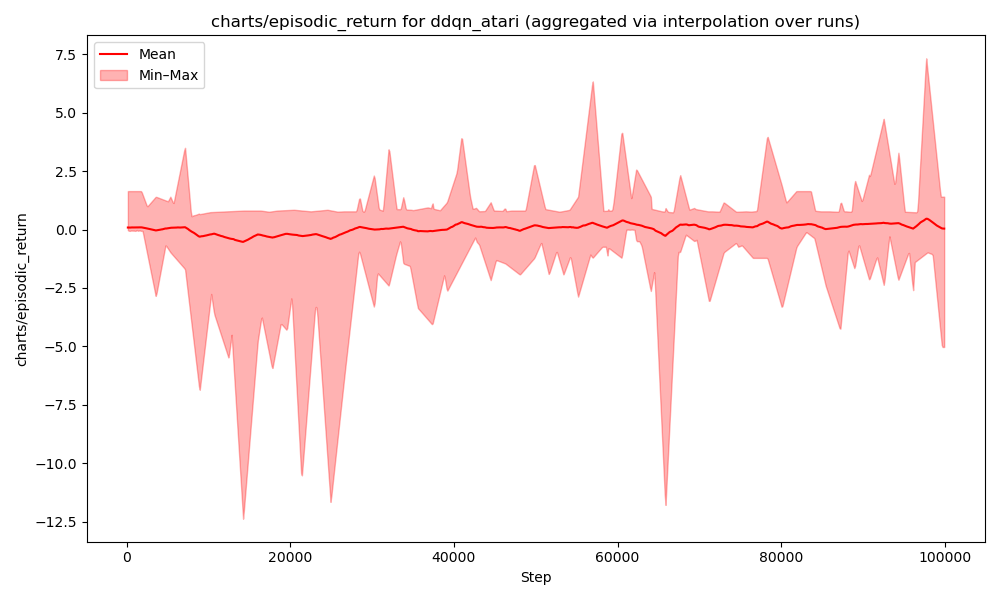
\includegraphics[width=0.6\textwidth]{figures/ddqn/charts_episodic_return_human_ddqn_atari.png}
	\caption{Double DQN episodic return (human-normalized), aggregated across 32 runs.}
	\label{fig:ddqn_return_human}
\end{figure}

\begin{figure}
	\centering
	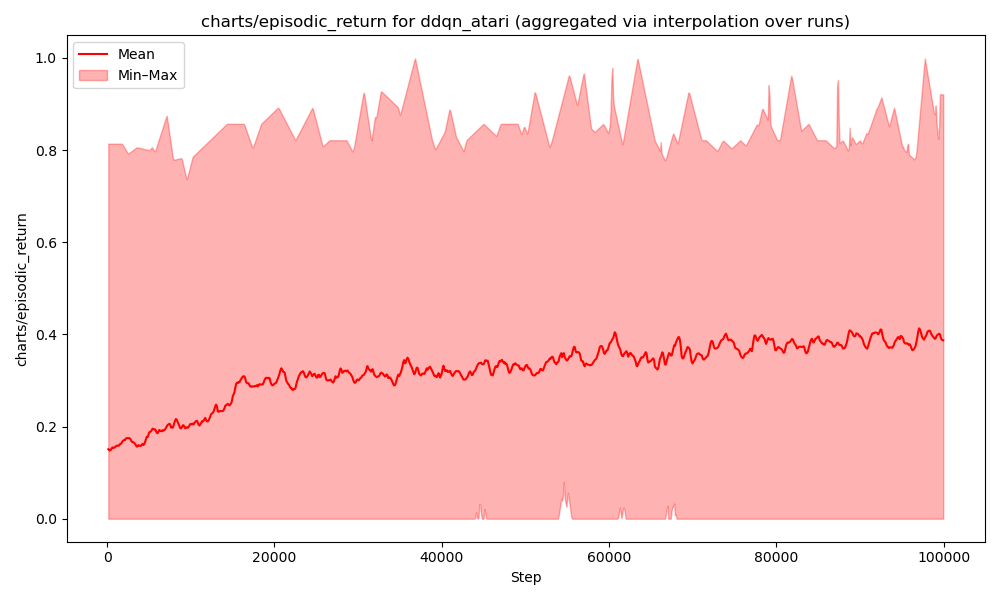
\includegraphics[width=0.6\textwidth]{figures/ddqn/charts_episodic_return_minmax_ddqn_atari.png}
	\caption{Double DQN episodic return (min--max normalized), aggregated across 32 runs.}
	\label{fig:ddqn_return_minmax}
\end{figure}

\begin{figure}
	\centering
	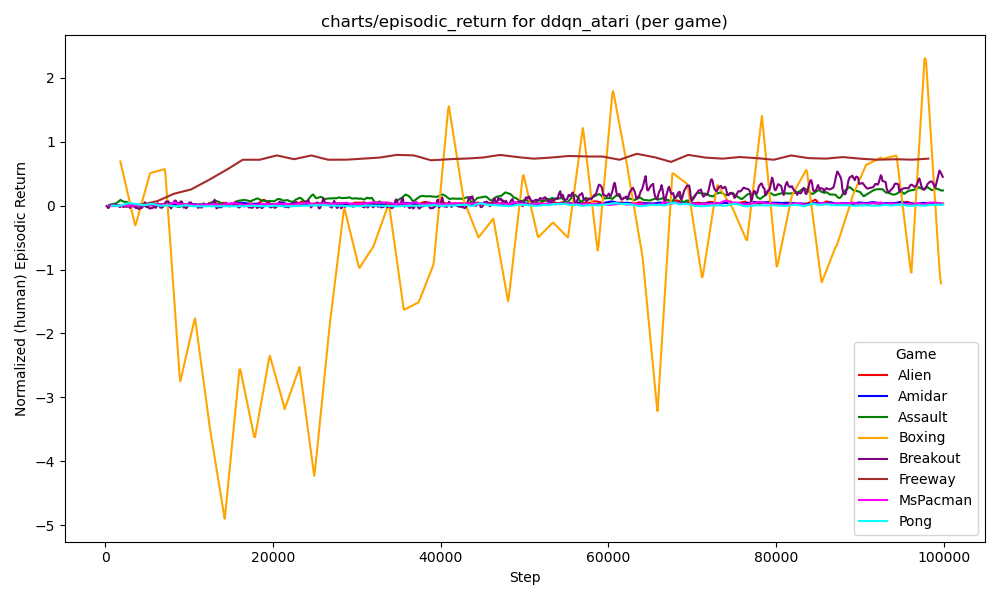
\includegraphics[width=0.6\textwidth]{figures/ddqn/charts_episodic_return_per_game_human_ddqn_atari.png}
	\caption{Double DQN returns per game (human-normalized). 
		Some large negative dips occur in \emph{Boxing}, 
		while \emph{Freeway} remains relatively high.}
	\label{fig:ddqn_return_pergame_human}
\end{figure}

\begin{figure}
	\centering
	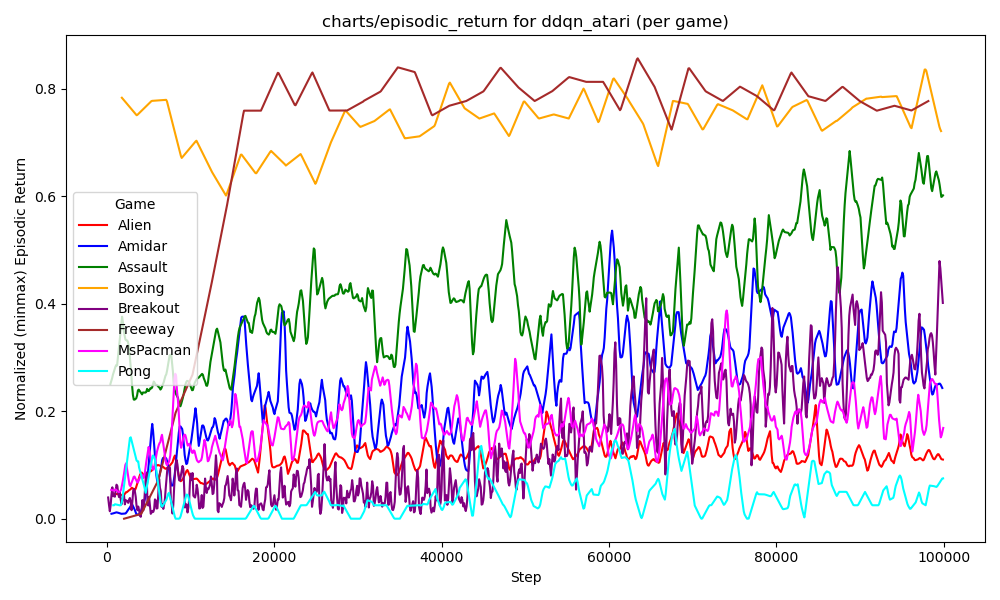
\includegraphics[width=0.6\textwidth]{figures/ddqn/charts_episodic_return_per_game_minmax_ddqn_atari.png}
	\caption{Double DQN returns per game (min--max normalized).}
	\label{fig:ddqn_return_pergame_minmax}
\end{figure}

As in the baseline, \emph{Freeway} can achieve near 0.7--0.8 in human norm, 
while \emph{Boxing} causes occasional highly negative runs. 
Min--max normalized returns rise from $\sim 0.2$ to $\sim 0.4$, 
similar to DQN’s overall trajectory.

\paragraph{Emissions.}
Table~\ref{tab:ddqn_emissions} summarizes Double DQN’s CO\textsubscript{2}-eq emissions across 32 runs. 
The mean is about \textbf{0.00667\,kg}, slightly above DQN’s \(\sim 0.00647\).

\begin{table}
	\caption{Carbon emissions (kg\,CO\textsubscript{2}eq) for Double DQN, aggregated over 32 runs.}
	\label{tab:ddqn_emissions}
	\centering
	\makebox[\textwidth]{%
	\begin{tabularx}{1.1\textwidth}{lXXXXXXXX}
		\toprule
		\textbf{Algorithm} & \textbf{mean} & \textbf{std} & \textbf{median} & 
		\textbf{q25} & \textbf{q75} & \textbf{min} & \textbf{max} & \textbf{iqmean} \\
		\midrule
		Double DQN & 0.006672 & 0.000282 & 0.006549 & 0.006477 & 0.006755 
		& 0.006377 & 0.007267 & 0.006565 \\
		\bottomrule
	\end{tabularx}
	}
\end{table}

\paragraph{Evaluation Results.}
Table~\ref{tab:ddqn_eval_overall} compiles final returns (human-/min--max normalization) aggregated over the 32 runs. 
Compared to DQN’s \(\sim\!0.135\) (human) and \(\sim\!0.380\) (min--max), Double DQN attains 0.023 (human) and 0.374 (min--max). 
While the min--max average is comparable, the human-normalized mean is noticeably lower due to substantial negative outliers (again, notably \emph{Boxing}).

\begin{table}
	\caption{Overall final evaluation (10 episodes each) for Double DQN across 32 runs.}
	\label{tab:ddqn_eval_overall}
	\centering
	\makebox[\textwidth]{%
	\begin{tabularx}{1.1\textwidth}{lXXXXXXXX}
		\toprule
		\textbf{Normalization} & \textbf{mean} & \textbf{std} & \textbf{median} & 
		\textbf{q25} & \textbf{q75} & \textbf{min} & \textbf{max} & \textbf{iqmean} \\
		\midrule
		\textbf{Human} & 0.0226 & 1.0083 & 0.0527 & 0.0127 & 0.2871 & -8.5952 & 2.5952 & 0.0894 \\
		\textbf{Min--Max} & 0.3737 & 0.2854 & 0.2887 & 0.1244 & 0.7054 & 0.0 & 1.0 & 0.3272 \\
		\bottomrule
	\end{tabularx}
	}
\end{table}

Table~\ref{tab:ddqn_eval_gamewise} shows the game-by-game breakdown, indicating \emph{Boxing} yields a min of -8.5952 and max of 2.5952 in human-normalized scale, dragging down the overall mean. Meanwhile, \emph{Freeway} remains consistently high.

\begin{table}
	\caption{Per-game final evaluation for Double DQN (human- vs.\ min--max normalized). 
		Each row aggregates 40 total episodes (10 per seed).}
	\label{tab:ddqn_eval_gamewise}
	\centering
	\begin{tabular}{llcccc}
		\toprule
		\textbf{Game} & \textbf{Norm} & \textbf{mean} & \textbf{std} & \textbf{min} & \textbf{max}\\
		\midrule
		Alien    & Human   & 0.0514 & 0.0340 & 0.0094 & 0.1327 \\
		& Min--Max & 0.1424 & 0.0565 & 0.0725 & 0.2775 \\
		\cmidrule{1-6}
		Amidar   & Human   & 0.0320 & 0.0222 & 0.0127 & 0.0953 \\
		& Min--Max & 0.2729 & 0.1708 & 0.1244 & 0.7604 \\
		\cmidrule{1-6}
		Assault  & Human   & 0.2310 & 0.1071 & -0.0427 & 0.4103 \\
		& Min--Max & 0.5913 & 0.1628 & 0.1754 & 0.8640 \\
		\cmidrule{1-6}
		Boxing   & Human   & -1.1607 & 2.4963 & -8.5952 & 2.5952 \\
		& Min--Max & 0.7227 & 0.0813 & 0.4806 & 0.8450 \\
		\cmidrule{1-6}
		Breakout & Human   & 0.2666 & 0.1470 & 0.0764 & 0.8738 \\
		& Min--Max & 0.2559 & 0.1165 & 0.1053 & 0.7368 \\
		\cmidrule{1-6}
		Freeway  & Human   & 0.7213 & 0.0493 & 0.6419 & 0.8784 \\
		& Min--Max & 0.7625 & 0.0521 & 0.6786 & 0.9286 \\
		\cmidrule{1-6}
		MsPacman & Human   & 0.0291 & 0.0245 & -0.0037 & 0.0730 \\
		& Min--Max & 0.1820 & 0.0986 & 0.0497 & 0.3586 \\
		\cmidrule{1-6}
		Pong     & Human   & 0.0100 & 0.0559 & -0.01 & 0.3233 \\
		& Min--Max & 0.0600 & 0.1676 & 0.0   & 1.0 \\
		\bottomrule
	\end{tabular}
\end{table}

\paragraph{Comparison with Baseline DQN.}
Beyond the final statistics, we can compare Q-values and TD loss directly via overlapping curves. Figure~\vref{fig:dqn_vs_ddqn_qvalues} shows the \texttt{losses/q\_values} for both algorithms, with \texttt{ddqn\_atari} in red and \texttt{dqn\_atari} in gold; Double DQN’s mean Q-values grow more slowly, suggesting less overestimation. Figure~\vref{fig:dqn_vs_ddqn_td_loss} indicates TD loss remains similarly small for both, though DQN occasionally spikes higher. The barplot in figure~\ref{fig:emissions_dqn_ddqn} shows the mean emissions side-by-side.

\begin{figure}
	\centering
	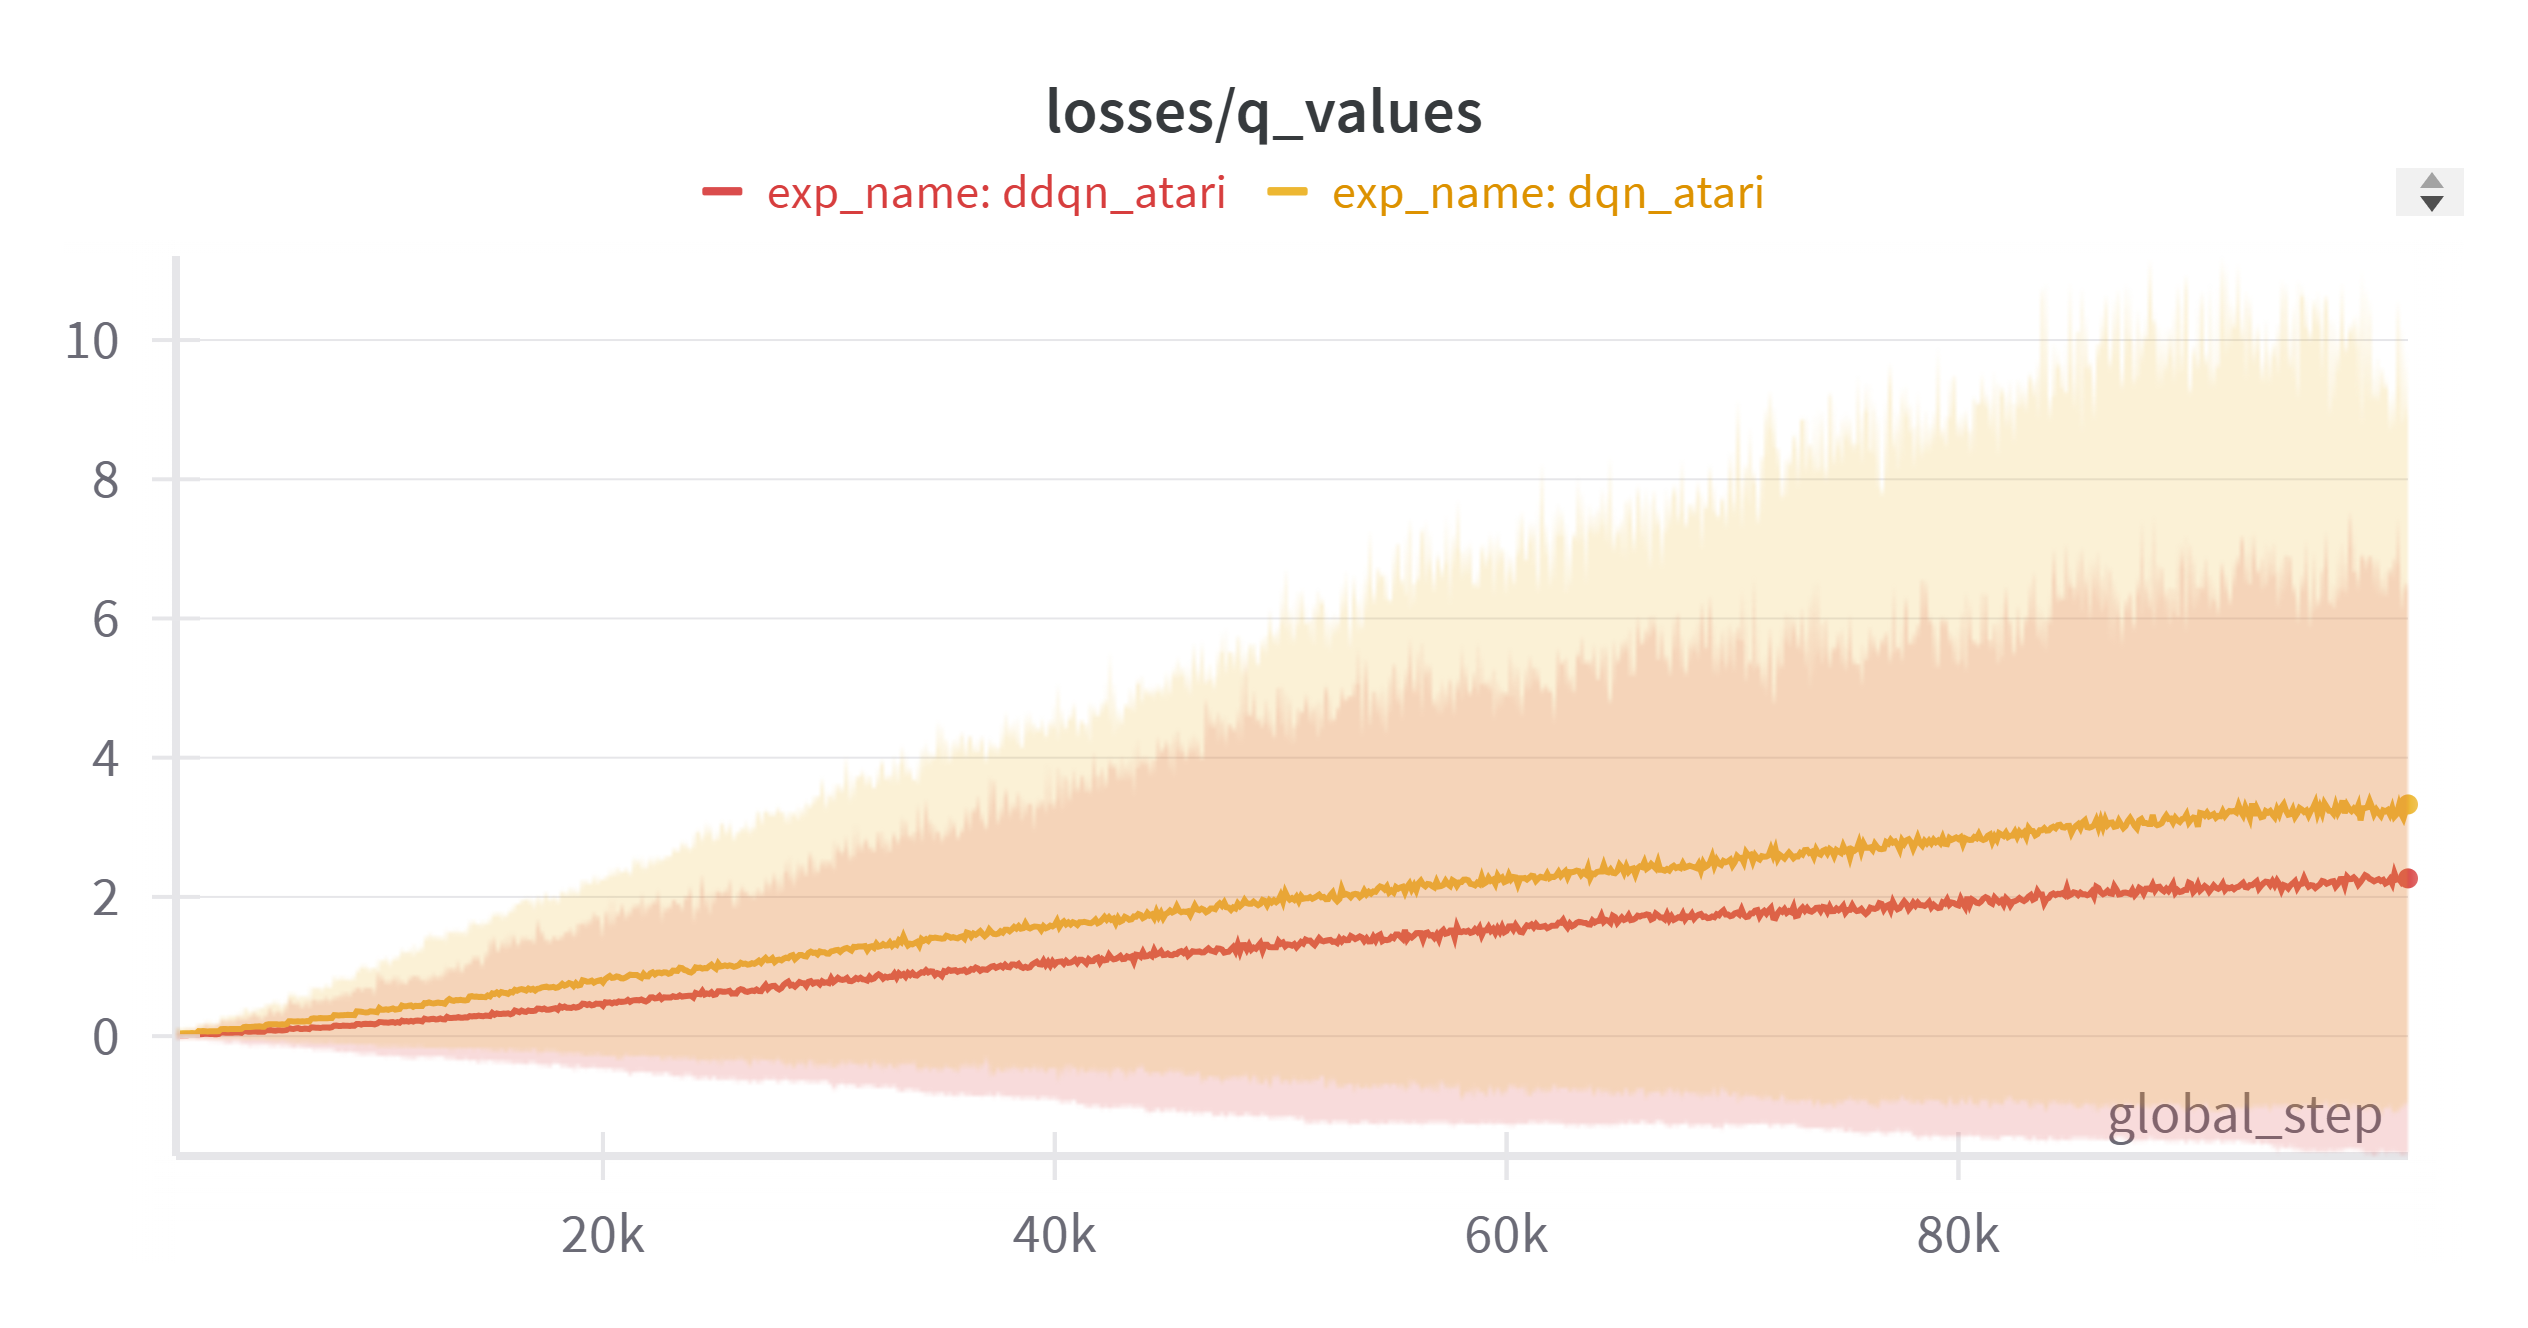
\includegraphics[width=0.6\textwidth]{figures/ddqn/comparison_losses_q_values_dqn_ddqn.png}
	\caption{Comparison of mean Q-values (with min--max shading) for DQN (gold) vs.\ Double DQN (red).}
	\label{fig:dqn_vs_ddqn_qvalues}
\end{figure}

\begin{figure}
	\centering
	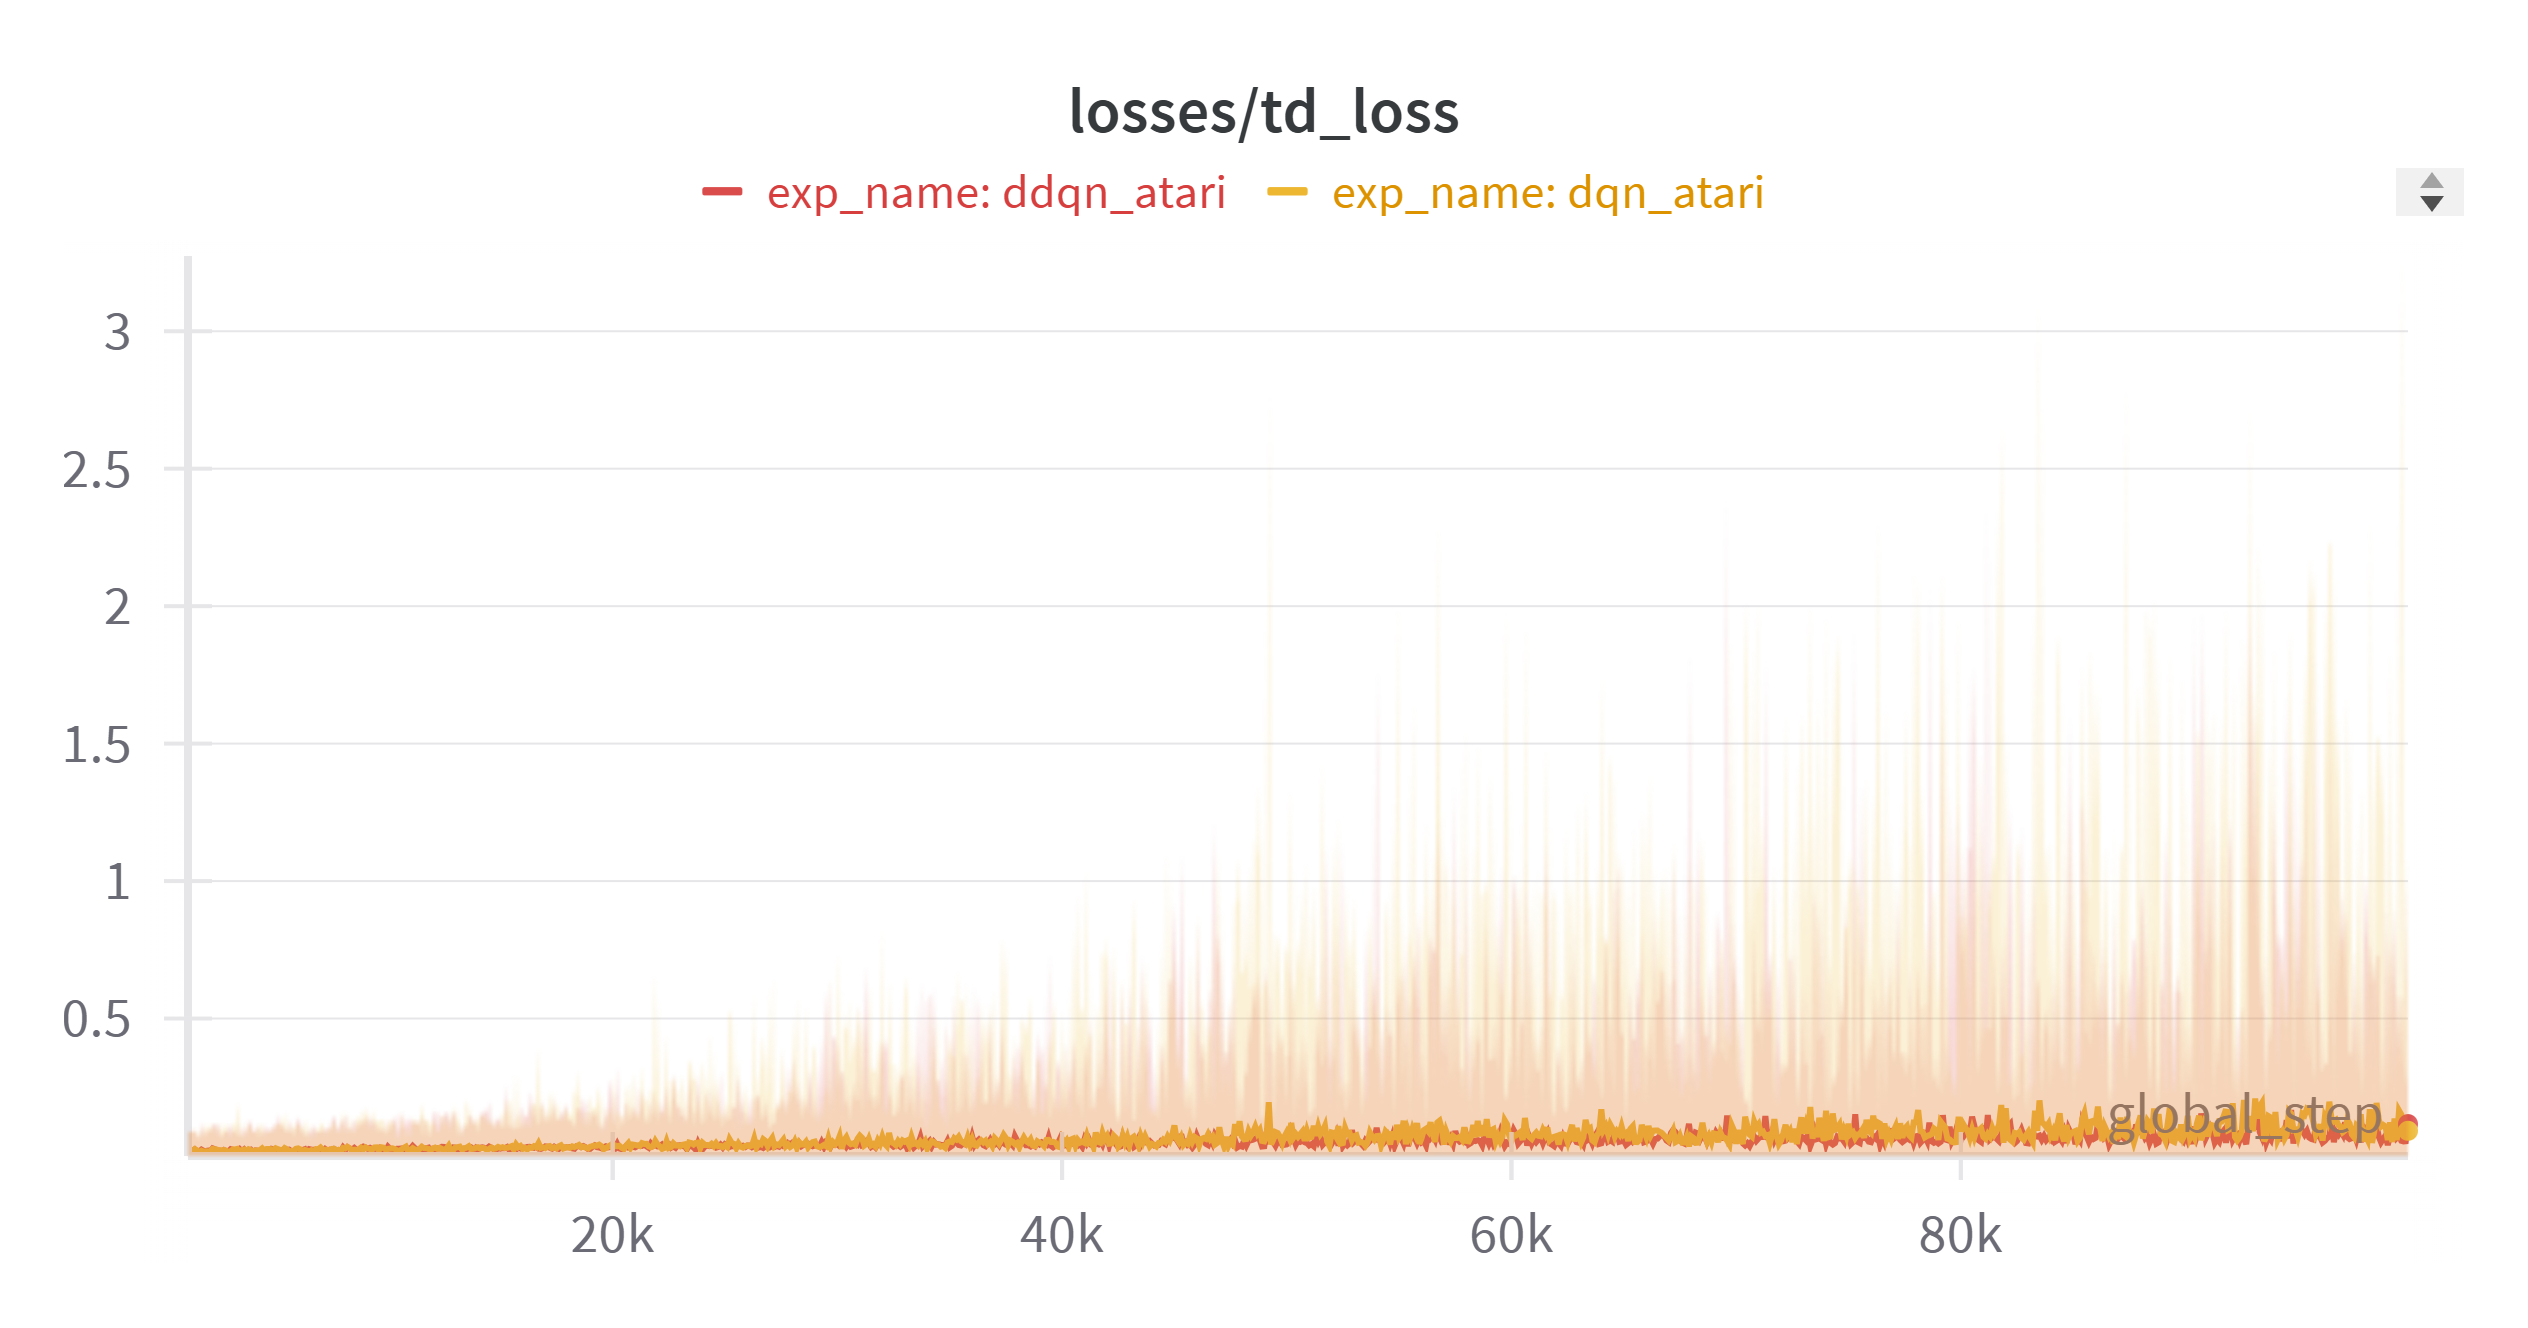
\includegraphics[width=0.6\textwidth]{figures/ddqn/comparison_losses_td_loss_dqn_ddqn.png}
	\caption{Comparison of TD loss for DQN (gold) vs.\ Double DQN (red). 
		Both remain near 0 for extended periods, though DQN shows slightly higher spikes.}
	\label{fig:dqn_vs_ddqn_td_loss}
\end{figure}


\begin{figure}
	\centering
	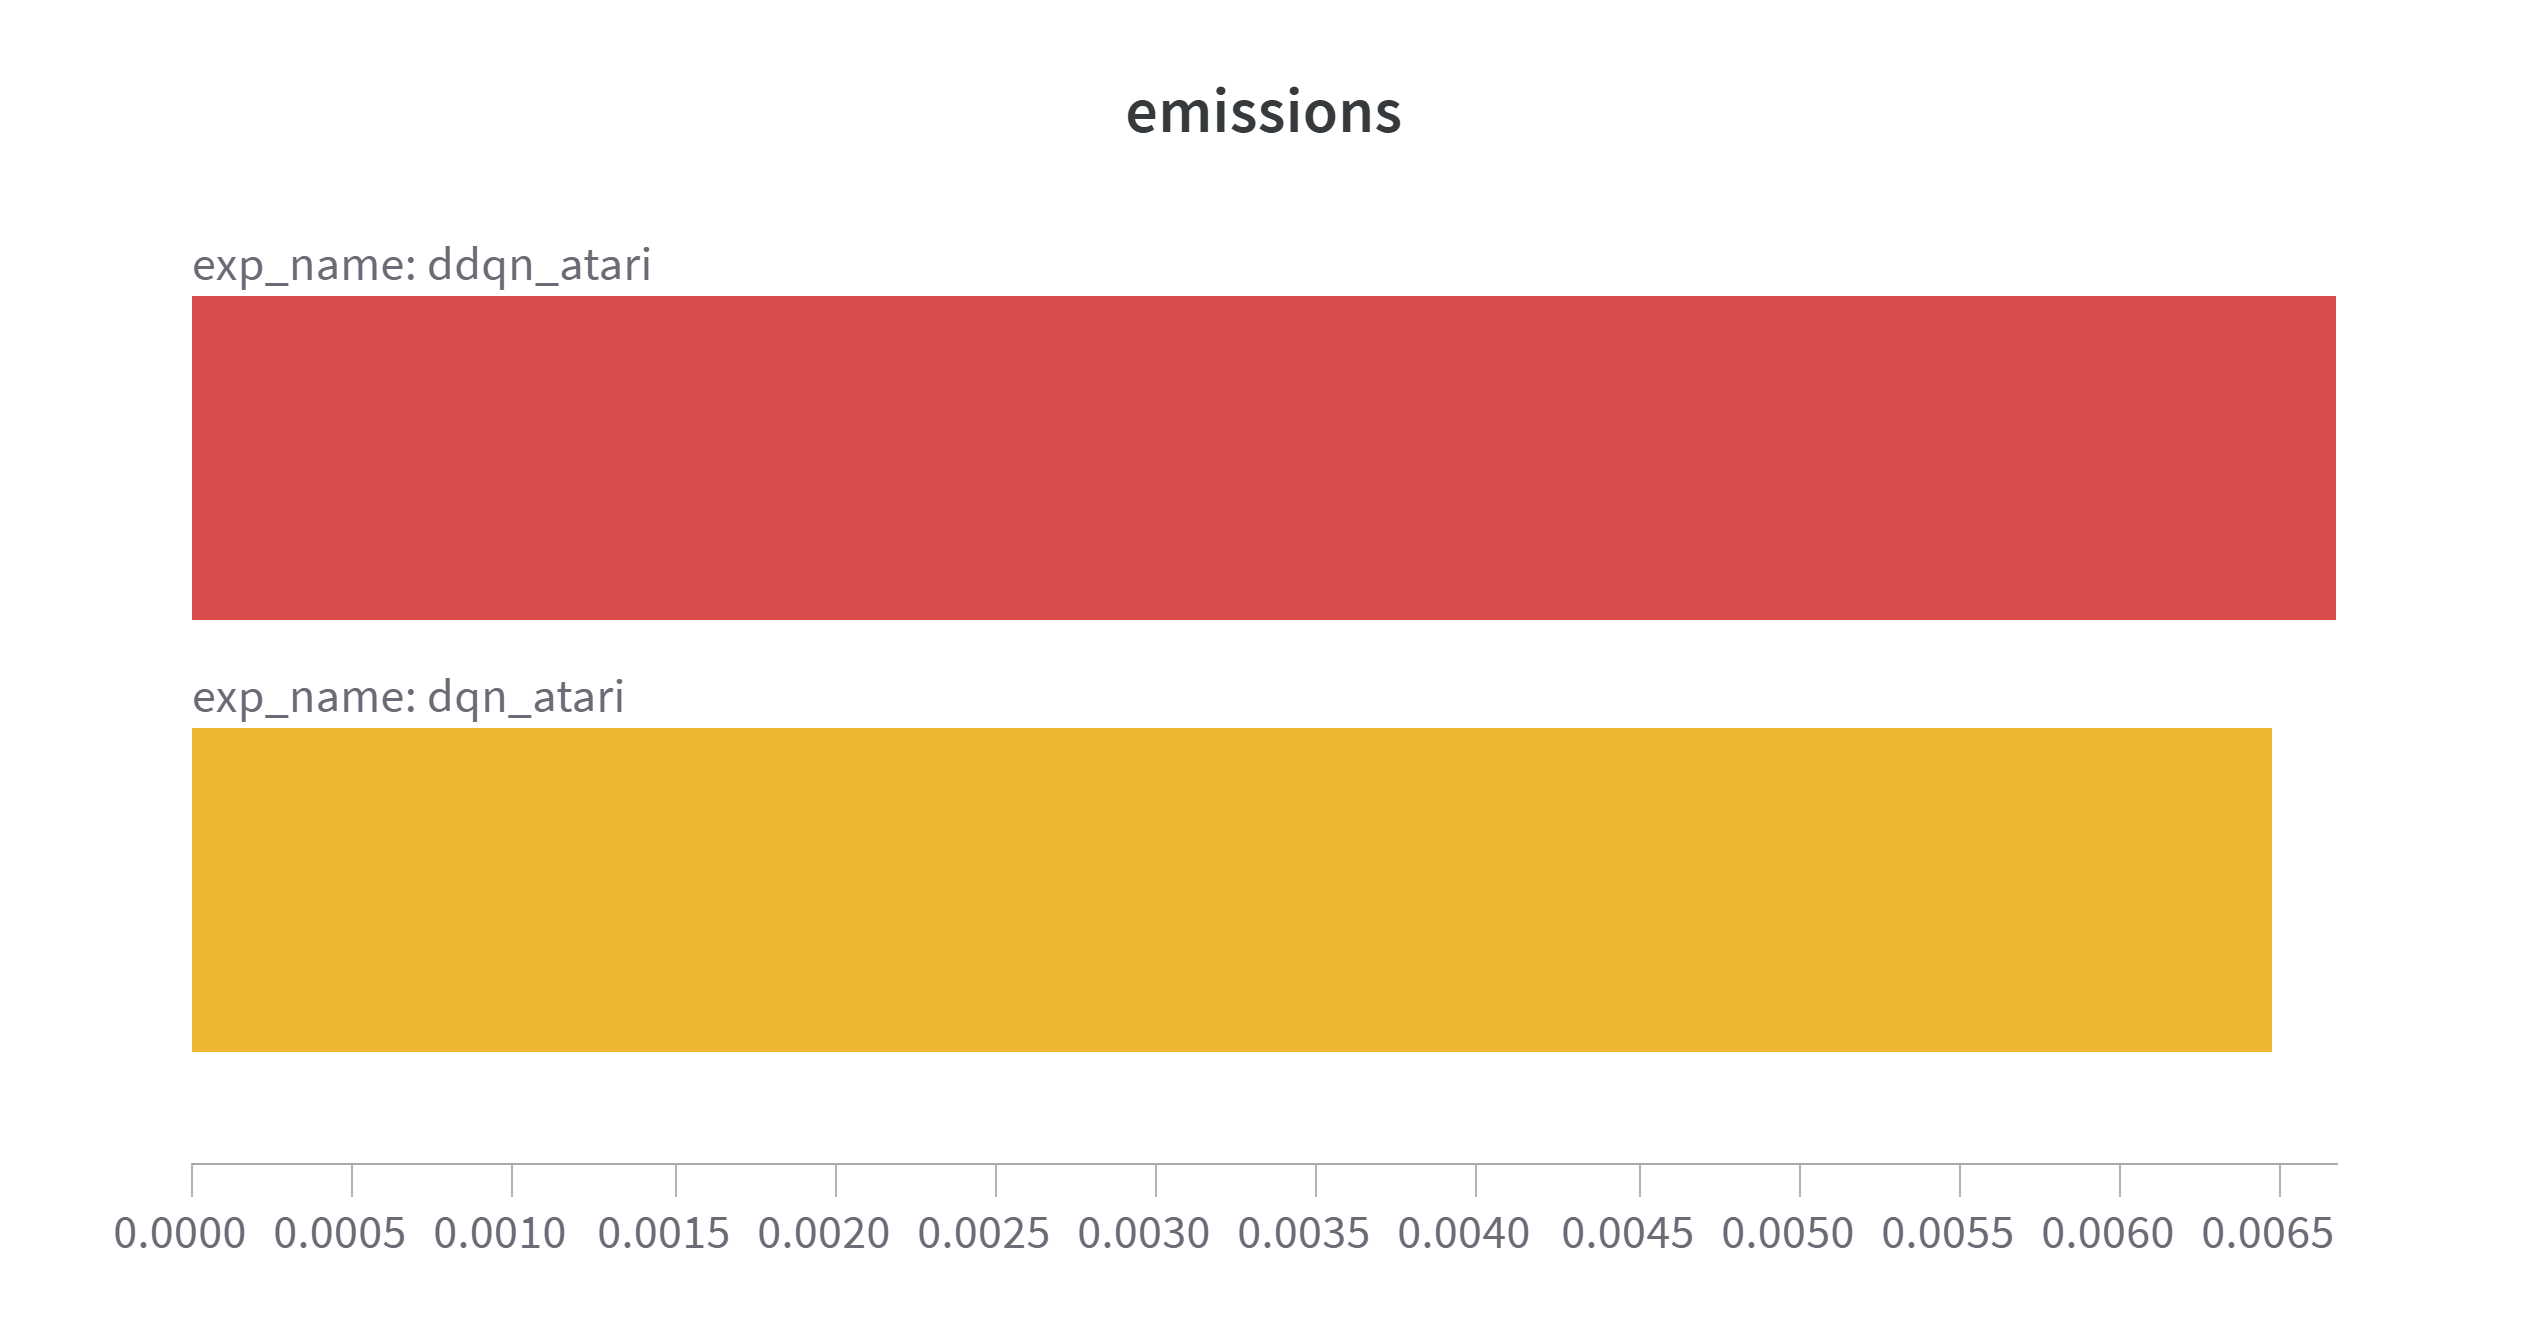
\includegraphics[width=0.6\textwidth]{figures/ddqn/emissions_dqn_ddqn.png}
	\caption{Mean emissions of DQN (gold) and Double DQN (red).}
	\label{fig:emissions_dqn_ddqn}
\end{figure}

Overall, Double DQN indeed moderates Q-value inflation compared to standard DQN, 
but under the 100k-step constraint, this reduction in overestimation does not strongly translate 
into consistently higher final returns.

\paragraph{Observations.}
\begin{itemize}
	\item \textbf{Q-values and Losses:} Double DQN’s Q-values peak lower than DQN’s (about 2--3 vs.\ 4--5), aligning with the bias-reduction theory. TD losses remain small for both algorithms, with occasional spikes.
	\item \textbf{Performance:} The min--max normalized mean (0.374) is nearly the same as DQN’s (0.380), while human-normalized is actually lower (0.023 vs.\ 0.135) due to certain highly negative runs, especially in \emph{Boxing}.
	\item \textbf{Emissions:} Average $\sim0.00667$\,kg CO\textsubscript{2}-eq, slightly higher than DQN’s $0.00647$\,kg.
\end{itemize}

Hence, although Double DQN successfully limits Q-value overestimation, its advantage does not 
fully manifest in higher aggregate returns at 100k steps—indicating that more extensive training 
or additional refinements may be needed to reap its potential performance gains.


\subsubsection{Prioritized Experience Replay}
\begin{itemize}
	\item How prioritization improved learning efficiency.
	\item Energy-performance trade-off compared to DQN and Double DQN.
\end{itemize}
Comparison with DQN and Double DQN.
Did it lead to better sample efficiency?
Energy consumption comparison.


\subsubsection{Dueling DQN}
\begin{itemize}
	\item Did dueling networks reduce variance?
	\item Performance and energy efficiency compared to other DQN methods.
\end{itemize}
Impact on stability.
Did it reduce variance in Q-value estimates?
Performance and energy trade-offs.


\subsubsection{C51 (Categorical DQN)}
\begin{itemize}
	\item Impact of distributional reinforcement learning.
	\item Did C51 improve sample efficiency?
\end{itemize}
Did distributional learning improve performance?
Energy efficiency vs. performance trade-off.


\subsection{Overall Comparison of DQN-Based Algorithms}
\begin{itemize}
	\item Graphs comparing all DQN-based methods.
	\item Summary table with:
	\begin{itemize}
		\item Final performance scores per game.
		\item Total training duration.
		\item Energy consumption.
	\end{itemize}
	\item Discussion: Which method offers the best balance between efficiency and performance?
\end{itemize}
Graphs comparing all 5 DQN-based algorithms on the same scale.
Tables summarizing:
Performance (average final score per game).
Training duration.
Total energy consumption.
Key takeaways: Which is the best energy-performance trade-off?

\subsection{Policy-Based Algorithms}
This section presents results for the three policy gradient methods.

\subsubsection{REINFORCE}
\begin{itemize}
	\item Training execution and stability.
	\item Performance scores and energy consumption.
\end{itemize}
Training execution.
Stability of policy gradient training.
Final scores and emissions.


\subsubsection{PPO (Proximal Policy Optimization)}
\begin{itemize}
	\item Effect of clipping on training stability.
	\item Performance vs. REINFORCE.
\end{itemize}
Did clipping help stabilize training?
Efficiency compared to REINFORCE.


\subsubsection{SAC (Soft Actor-Critic)}
\label{subsubsec:sac}
\begin{itemize}
	\item Impact of entropy regularization.
	\item Energy efficiency compared to PPO and REINFORCE.
\end{itemize}
How did the entropy regularization affect performance?
Energy trade-offs (is SAC more expensive to train?).


\subsection{Overall Comparison of Policy-Based Algorithms}
\begin{itemize}
	\item Graphs comparing all policy-based methods.
	\item Which method achieved better stability?
	\item Summary of trade-offs between energy consumption and performance.
\end{itemize}
Graphs comparing policy-based methods.
Which is more stable? Which is more efficient?
Final takeaway: Did one clearly outperform the others in both energy efficiency and reward?


\subsection{Cross-Category Comparison: DQN vs. Policy Gradient}
\begin{itemize}
	\item Which family was more energy-efficient?
	\item Graphs comparing the best-performing models from each category.
	\item Conclusion: Do policy-based methods require more energy but provide better sample efficiency?
\end{itemize}
Which family is generally more energy-efficient?
Graphs comparing best DQN-based vs. best policy-based model.
Final summary of the findings.